\section{Results}

We tested our method with an Intel Pentium 3550M processor and a NVIDIA GeForce GTX 850M GPU. 
We implemented it with C++ and GLSL. 
The pipeline runs with geometry shaders, combined with transform feedbacks. 

\paragraph{}
We ran our method on different volumetric datasets.
The first one is a stack-based representation of a terrain, called Moria, created with the ARCHES framework \cite{peytavie2009arches}.
It contains $512^3$ voxels, which we uploaded on the GPU using a 3D texture.
We also used two other datasets to further illustrate the performances of our method.
We first visualised a set of metaballs.
Those implicit surfaces are defined analytically to be evaluated on the GPU and are updated at every frame.
This scene creates objects that goes through high geometrical changes and thus cannot be precomputed.
We also visualised an animated ocean.
This object is again defined analytically and evaluated on the GPU. 
All those scenes are illustrated in Figure \ref{final_outputs} and in the accompanying video.

\paragraph{}
In all our experiments, we used the LoD criterion given in equation (\ref{improved_lod_criterion}).
This criterion is data parallel and is based on the projected size of the cells.
It thus prevents rasterization under-sampling and can be efficiently used on the GPU (Figure \ref{lod})

\begin{figure}
\centering
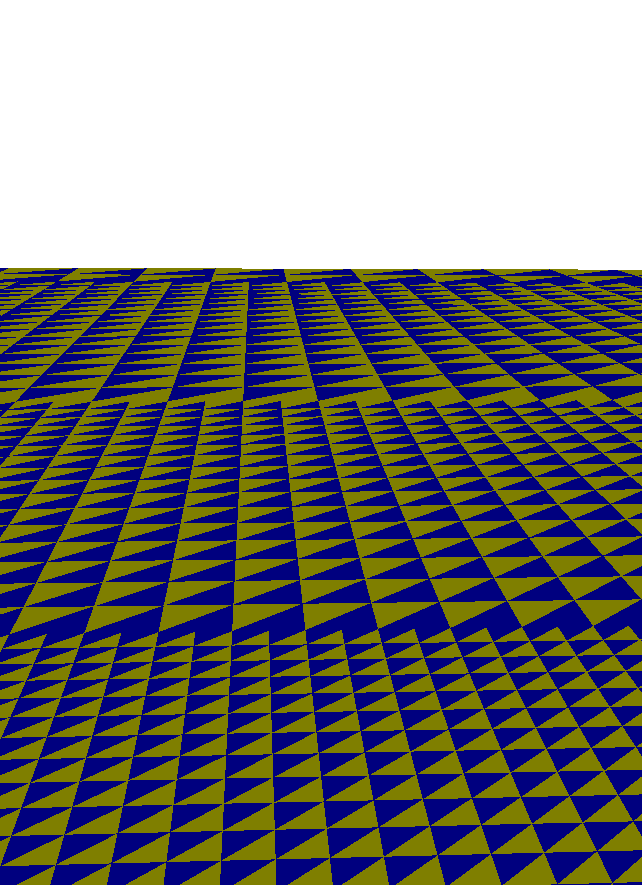
\includegraphics[height=0.2\textheight]{alias}
\hfill
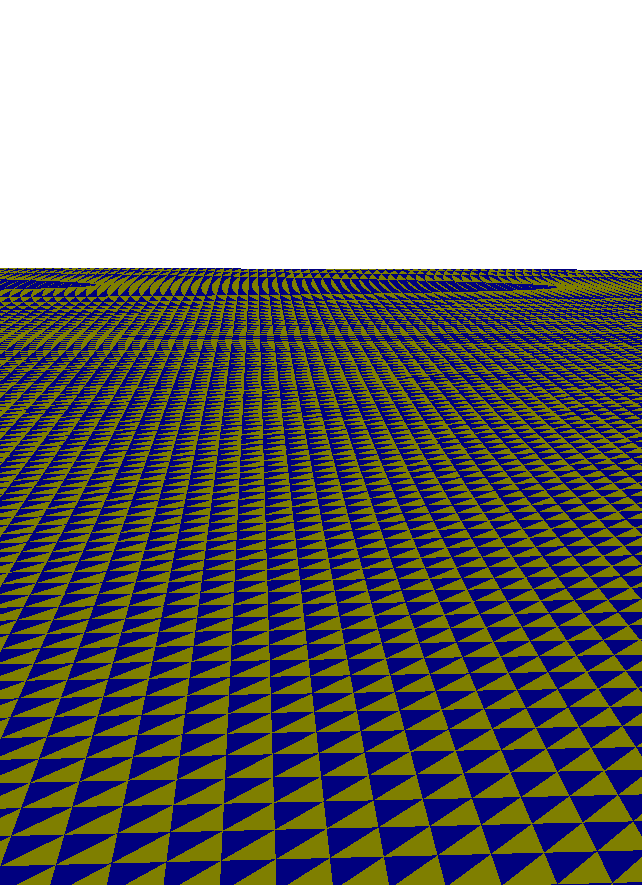
\includegraphics[height=0.2\textheight]{filtered}
\caption{Each extracted triangle has a different color. (Right) presents the result of rasterizing an object visualised with a regular grid. (Left) presents the result of rasterizing an object visualised with our LoD criterion. It can be seen that the aliasing artefacts present on (Right) disappeared on (Left).}
\label{lod}
\end{figure}

\subsection{Stack-based terrain}

\paragraph{}
We ran our method on the Moria scene \cite{peytavie2009arches}, enhanced with a noise function to add high resolution geometric details.
We present the average execution times for each step of the pipeline, as well as the number of cells in input (Table \ref{table_step}).

\begin{table}[tb]
\centering
\begin{tabular}{|l|c|c|c|}
\hline
Step           & Time (ms) & \#Cells & Memory (MB) \\ \hline
Update         & 1.13      & 219295  & 1.67        \\
Culling        & 3.3       & 219295  & 1.67        \\
Triangulation  & 0.94      & 5570    & 0.04        \\ \hline
Total GPU time & \multicolumn{3}{c|}{5.4}           \\ 
Total CPU Time & \multicolumn{3}{c|}{2.3}          \\ \hline
\end{tabular}
\caption{Average execution time for each step of the pipeline during a flythrough of the Moria scene.
The first column gives the average execution time, 
the second contains the number of cells in input, and
the last gives the memory size of the buffer used.
Since each cell is coded on 64 bits, the memory footprint of a buffer is $\mathrm{buffer\_size} * 64$ bits.}
\label{table_step}
\end{table}

\paragraph{}
We can note that updating the octree is very fast (less than 2 ms) whereas the culling step is slower (by roughly 300\%).
This is due to the fact that this pass runs tests on the whole partition, which can be computationally expensive.
Nonetheless, this efficient culling allows the triangulation to run on a very small amount of cells, thus reaching very good performances.
Finally, the total GPU time needed to update and triangulate the new frame is under 6 ms (180 FPS), for a memory consumption of only 4 MB.
Furthermore, as every computation is done on the GPU, the CPU is only active for 2 ms to initiate the shaders.

\subsection{Animated metaballs}

\paragraph{}
The cells inside the frustum are re-triangulated at each frame.
Therefore, it is possible to visualise fully dynamic data without any performance loss.
We tested this while visualising animated metaballs.
When running our experiments, the animation was stopped between the frames 5000 and 10000.
We can then show that our framerate is not affected by the changes in the scene.
The camera was static during the whole experiment to remove all variability that would have been induced if the number of cells to evaluate was changing.
The resulting graph is shown in Figure \ref{metaballs_graph}.

\begin{figure}
\centering
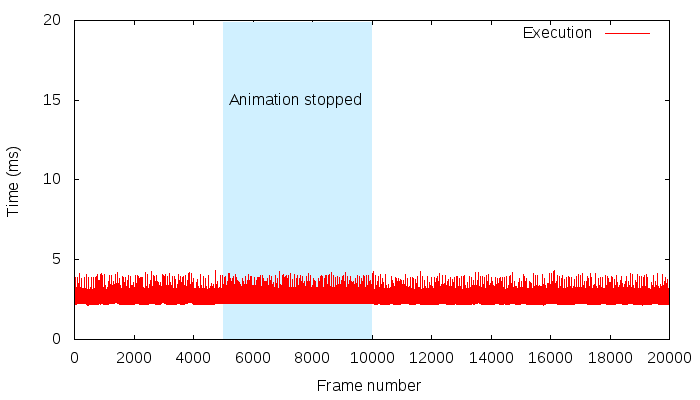
\includegraphics[width=\linewidth]{l_importance_d_etre_constant}
\caption{Rendering time for an animated scene. 
The average rendering time is about 3 ms even though the object is re-triangulated on each frame.
Those timings do not include the shading.
The blue box identifies the frames during which the object was static.
As can be seen, the fact that the object is or not animated has no impact whatsoever on the rendering time.}
\label{metaballs_graph}
\end{figure}

\paragraph{}
As can be seen on this graph, the triangulation timings are constant.
The only variability that can be measured is induced by the task scheduling on the GPU.


\subsection{Comparison}

%\paragraph{}
%Our goal in this work is to get a correct visualisation as fast as possible.
%The surface is triangulated for rasterization purposes and is not kept in memory.
%This differs from other methods that focuses on the topology of the mesh and return a full mesh.
%Furthermore, we gave ourselves the constraint that this method should be completely data parallel.
%This condition allows us to present a full GPU implementation with very high framerates.
%From those, we can afford to re-triangulate the whole object on the fly and still do a real-time visualisation.
%This differentiate our solution from most methods that achieve real-time through pre-process and data caching.

\paragraph{}
As developed during the introduction, there are several kind of methods on the state of the art.
The first category focuses on extracting a complete mesh from the data and are thus slower than methods that aim only at visualisation.
Amongst the visualisation solutions, the real-time is mostly achieved with data caching and pre-processing.
Here, we constrained ourselves to run in real-time without this data-caching and pre-processing, by taking full advantage of the GPU.
The solutions developed by other methods are thus quite different from ours.

\paragraph{}
We present a completely data parallel implementation based on the method of Lengyel \textit{et al}. \cite{lengyel2010voxel}.
Therefore, a pertinent comparison to prove our solution would be to compare both algorithms.
Since the method of Lengyel \textit{et al}. is part of a commercial game engine, it is not freely accessible.
We used instead a free implementation, independently developed by Lanner \cite{lanner}.
This implementation is based on data-caching.
The volumetric object is pre-triangulated at every level of detail during a preprocess.
Therefore during rendering, the only task left is to identify the cells of the octree's active front and to send their pre-computed triangulation to the GPU.
This increases the rendering speed but the preprocessing time can be prohibitive.
Furthermore, it is memory intensive.
Still, this implementation is very fast and allows localized modifications of the data.

\paragraph{}
We ran both methods on a static voxel based scene, adapting the LoD criteria to have a similar behaviour.
The dataset has a resolution of $256^3$.
The results are given in Figure \ref{cpu_gpu}.
It can be seen on this graph that even though we re-triangulate the cells at each frame, we are still running faster than a CPU implementation.
Furthermore, there is no transfer between the CPU and the GPU in our implementation.
This give us a speed up over CPU implementations that are constantly transferring data to the GPU.

\begin{figure}
\centering
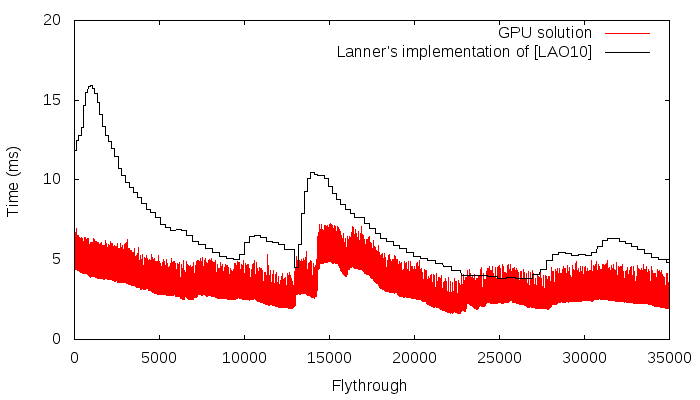
\includegraphics[width=\linewidth]{cpu_gpu}
\caption{Comparison between our GPU solution and Lanner's implementation \cite{lanner}.
This graph presents the execution time in ms for each frame.
}
\label{cpu_gpu}
\end{figure}


\begin{figure*}
\centering
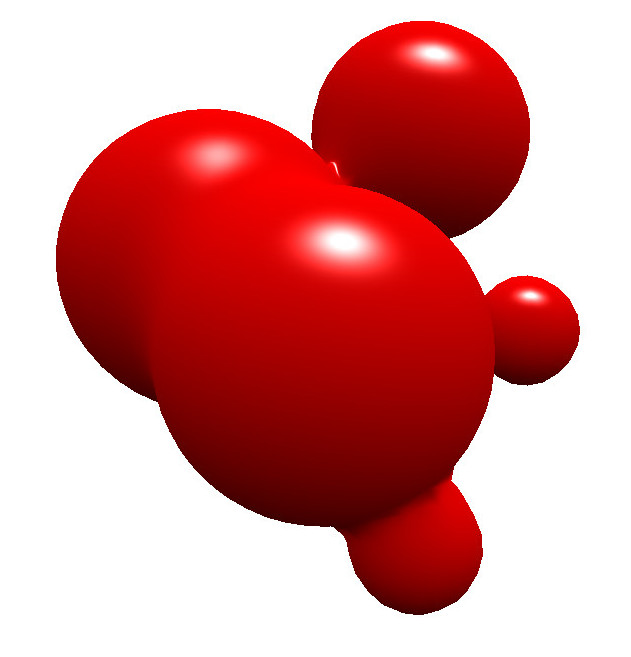
\includegraphics[height=0.17\textheight]{metaballs}
\hfill
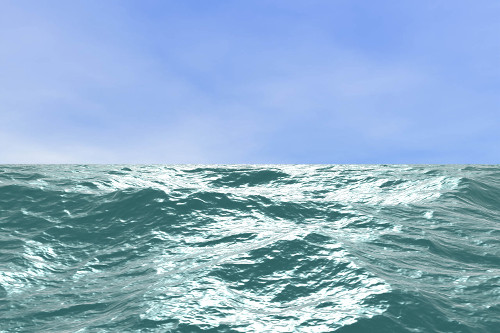
\includegraphics[height=0.17\textheight]{ocean}
\hfill
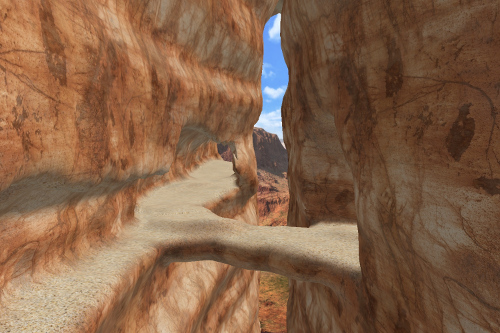
\includegraphics[height=0.17\textheight]{moria2}
\caption{This shows some outputs of our program. (Left) is an example of moving metaballs. (Middle) is an animated ocean. (Right) is a stack based terrain from the ARCHES plateform \cite{peytavie2009arches} }
\label{final_outputs}
\end{figure*}
